\chapter{RESULTS}
\label{chapter:results}

\section{The Bean V2 prototype Implementation}
The Bean V2 prototype was designed for a standard 180-nm CMOS process. This iteration of the Bean includes two standalone structures: a trimmed version a readout channel, which includes two CSA (one to generate the baseline\footnote{The baseline is defined as the CSA DC output voltage after reset, when no input has been applied.} voltage), a pre-charger circuit, the designed SC filter and output buffers; and an isolated version of the filter with its inputs directly bonded out off-chip.  Both structures will be tested separately, thus control signals and reference voltages for both filters are tied together. Also, a logic circuit to generate the non-overlapping two-phase clock was included. Future revisions of the Bean will include an ADC within the channel.

Fig.~\ref{fig:IC_layout} shows the layout of the Bean V2 prototype; for a detailed description of the IC pinout, see Apprendix~A. Each channel cell was designed to have a pitch lower than $190\,\mu\text{m}$. If the number of channels is increased to the nominal value of 32, the IC will be approximately 6~mm tall, which can be fit into four UMC180 mini@sic sub-blocks according to the Europractice rules. After including the ADC and the digital memory, channel length is expected to be lower than $1\,\text{mm}$.

The SC filter, shown in Fig.~\ref{fig:filter_layout}, has a total area of $185\,\mu\text{m}\times 332\,\mu\text{m}$, and was layout to resemble the components spatial distribution of circuit in Fig.~\ref{fig:filter_post}. The filters outputs, the main CSA output and the baseline voltage are buffered out off-chip using the rail-to-rail amplifiers (connected as unity-gain buffers) shown in Fig.~\ref{fig:buffer_layout}. The CSA and the filter OTA are depicted in Figs.~\ref{fig:csa_layout} and \ref{fig:ota_layout} respectively. All structures were carefully side-shielded with multiple guard-rings. Also, to mitigate the effects of cross-chip gradients,  common centroid layout and dummy devices were used in the layout of the filter OTA and the rail-to-rail op-amps. These considerations were not taken into account for the CSA layout, since mismatch is not critical for this cell because of the size of its transistors and also because it is single-ended. As mentioned in the previous chapter, $C_F$ and $C_S$ capacitors were implemented with a parallel connection of unity capacitors. To prevent copper-dishing effects, both capacitors were surrounded by dummy capacitors implemented with the same unitary capacitors.

Because of the lack of models for the pads provided by Faraday and the tools needed to use them, it was necessary to design custom pads. They were designed for ground, positive supply voltage, analog input/output, digital input, and digital output. Special care was taken for the Latch-up failure of the output digital drivers, and the Electrostatic discharge phenomena. 


\begin{figure}[!t]
	\centering
	\includegraphics[width=5in]{./Figures/IC_layout}
	\caption{The Bean 2 prototype layout.}\label{fig:IC_layout}
\end{figure}


\begin{figure}[!t]
	\centering
	\includegraphics[width=6in]{./Figures/filter_layout}
	\caption{Filter Layout.}\label{fig:filter_layout}
\end{figure}


\begin{figure}[!p]
	\centering
	\includegraphics[width=4in]{./Figures/CSA_layout}
	\caption{Charge-sensitive amplifier layout.}\label{fig:csa_layout}
\end{figure}

\begin{figure}[!t]
	\centering
	\includegraphics[width=4.5in]{./Figures/OTA_layout}
	\caption{Recycling folded cascode OTA layout.}\label{fig:ota_layout}
\end{figure}

\begin{figure}[!t]
	\centering
	\includegraphics[width=4.5in]{./Figures/buffer_layout}
	\caption{Rail-to-rail operational amplifier layout.}\label{fig:buffer_layout}
\end{figure}


\section{Filter post-layout simulation results}
\subsection{Power dissipation} 

The power dissipated by the SC filter prototype was calculated using transient simulations over the extracted filter, under nominal operation and a single input value. The results are presented in Table~\ref{tab:power_dissipation}, the measurements are current consumption averages of the supply node of each component. 

\begin{table}
	\begin{center}
		\begin{tabular}{|l|c|}\hline
			{\bf Component} & {\bf Current dissipation} \\ \hline\hline
			%CSA & $2.718\,\text{mW}$ \\ \hline			
			%CSA bias & $0.954\,\text{mW}$ \\ \hline			 
			Filter OTA & $369\,\mu\text{A}$ \\ \hline
			Filter bias and logic & $194\,\mu\text{A}$ \\ \hline
			Unitary-gain buffer & $360\,\mu\text{A}$ \\ \hline
		\end{tabular}
		\vspace*{5pt}
		\caption{SC filter simulated current dissipation.}
		\label{tab:power_dissipation}
	\end{center}
\end{table}

\subsection{Sub-blocks}
\subsection{Functionality} 
\subsection{Linearity}
\subsection{Weighting function}
The filter weighting function (WF) was measured according to its definition described in Chapter~\ref{chapter:theoretical}. This was done by applying an input voltage step at different times within a cycle, and measuring the output at the measurement time. A simple $RC$ network was used to simulate a realistic voltage step. Fig.~\ref{fig:wf_test_circuit} shows the circuit used to perform this measurement. 

Fig.~\ref{fig:sim_wf} shows the post-layout SPICE-simulated WF of the filter using plain coefficients and the Bean nominal clock frequency. As expected its shape resembles the shape of the WFs in Fig.~\ref{fig:optimum_wf}. Although the filter exceeds the settling time specification, 

 As explained before, the filter does not reach required settling time 

\begin{figure}[!t]
	\centering
	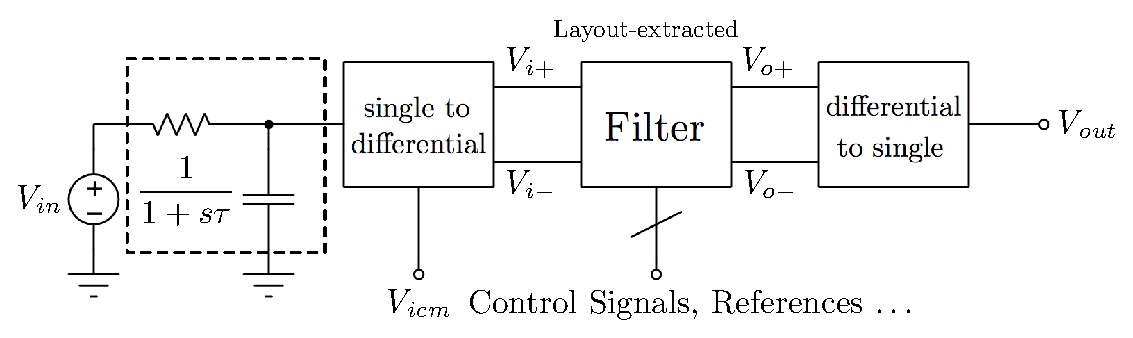
\includegraphics[width=5in]{./Test/wf_test_circuit}
	\caption{Weighting function test circuit.}\label{fig:wf_test_circuit}
\end{figure}

\begin{figure}[!t]
	\centering
	\includegraphics[width=3.6in]{./Test/sim_wf}
	\caption{SPICE-simulated weighting function. $\tau=8\,\text{ns}$, $N=16$ and $T_s=19.25\,\text{ns}$.}\label{fig:sim_wf}
\end{figure}

To characterize the designed filter and 
\begin{figure}[!t]
	\centering
	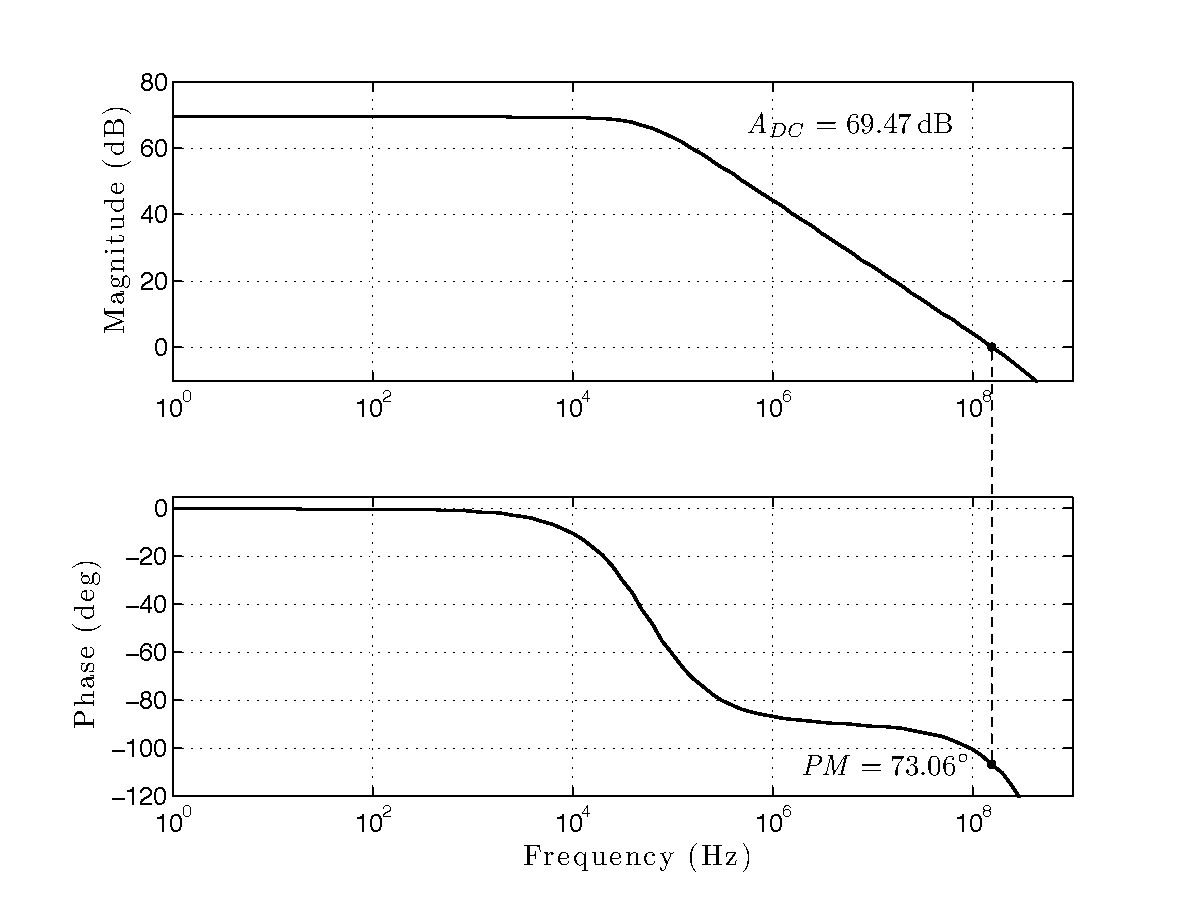
\includegraphics[width=5.3in]{./Test/bode_OTA_post}
	\caption{Bode plot for the OTA open-loop response.}\label{fig:bode_OTA}
\end{figure}


\begin{figure}[!t]
	\centering
	\includegraphics[width=4.4in]{./Test/gain_curves.pdf}
	\caption{Filter output step response with the 64 programmable gains. \mbox{$V_\textit{in}=0.1\,V$} and \mbox{$T_s=40\,\text{ns}$}.}\label{fig:gain_curves}
\end{figure}

\begin{figure}[!t]
	\centering
	\includegraphics[width=4.4in]{./Test/linearity.pdf}
	\caption{Filter linearity test results, full-scale input range.}\label{fig:gain_curves}
\end{figure}


\begin{figure}[!t]
	\centering
	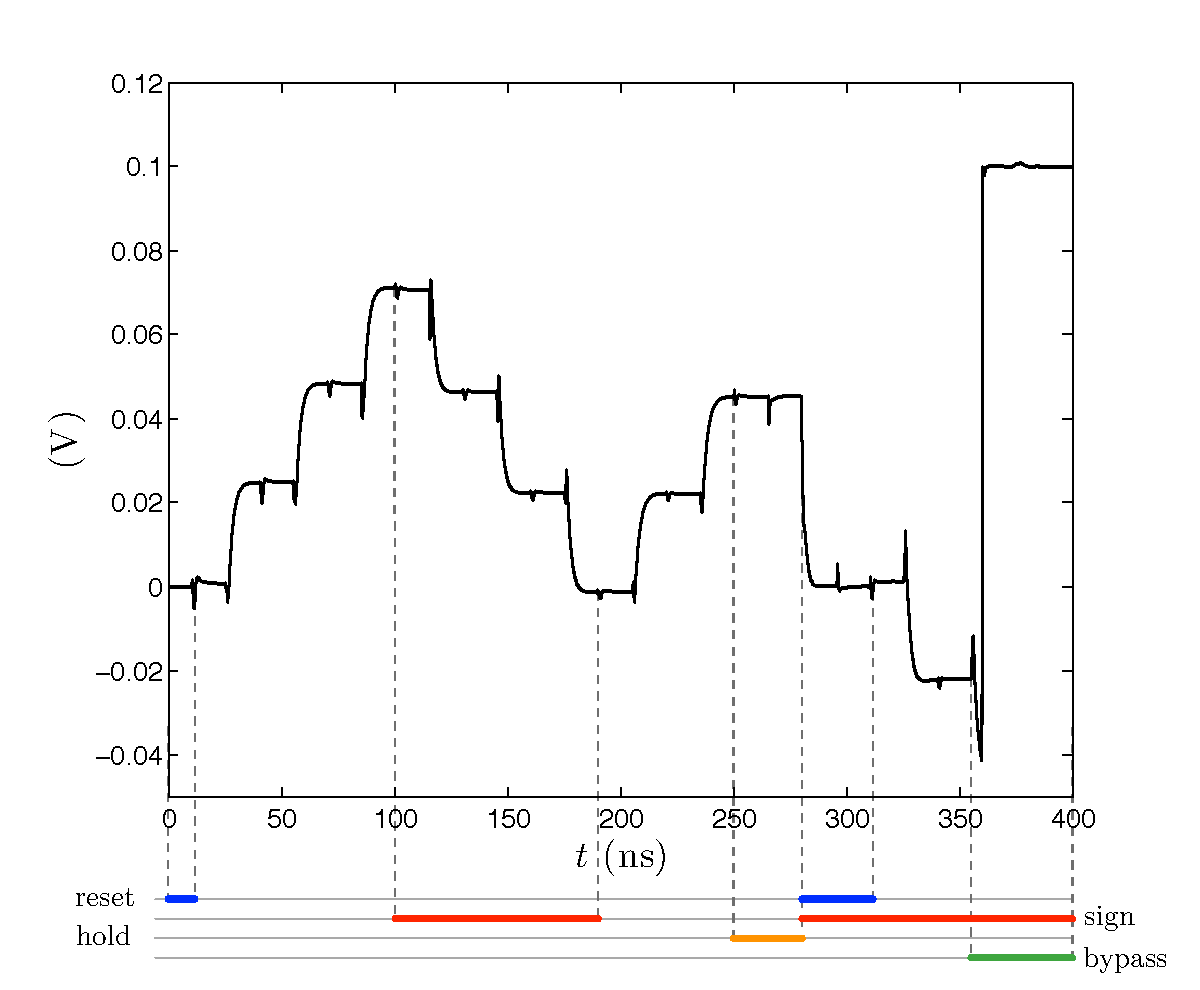
\includegraphics[width=5in]{./Test/test_filter_after_omni.eps}
	\caption{Filter control signals testing. $V_\textit{in}=0.1\,V$ and $\text{gain}=0.25\,V/V$.}\label{fig:test_filter_after_omni}
\end{figure}




\begin{figure}[!t]
	\centering
	\includegraphics[width=5.3in]{./Test/bode_buffer_post}
	\caption{Bode plot for the buffer open-loop response.}\label{fig:bode_buffer}
\end{figure}